\documentclass{ximera}

\begin{document}
	\author{Stitz-Zeager}
	\xmtitle{Exercises for Polar Graphs}{}

\mfpicnumber{1} \opengraphsfile{ExercisesforPolarGraphs} % mfpic settings added 

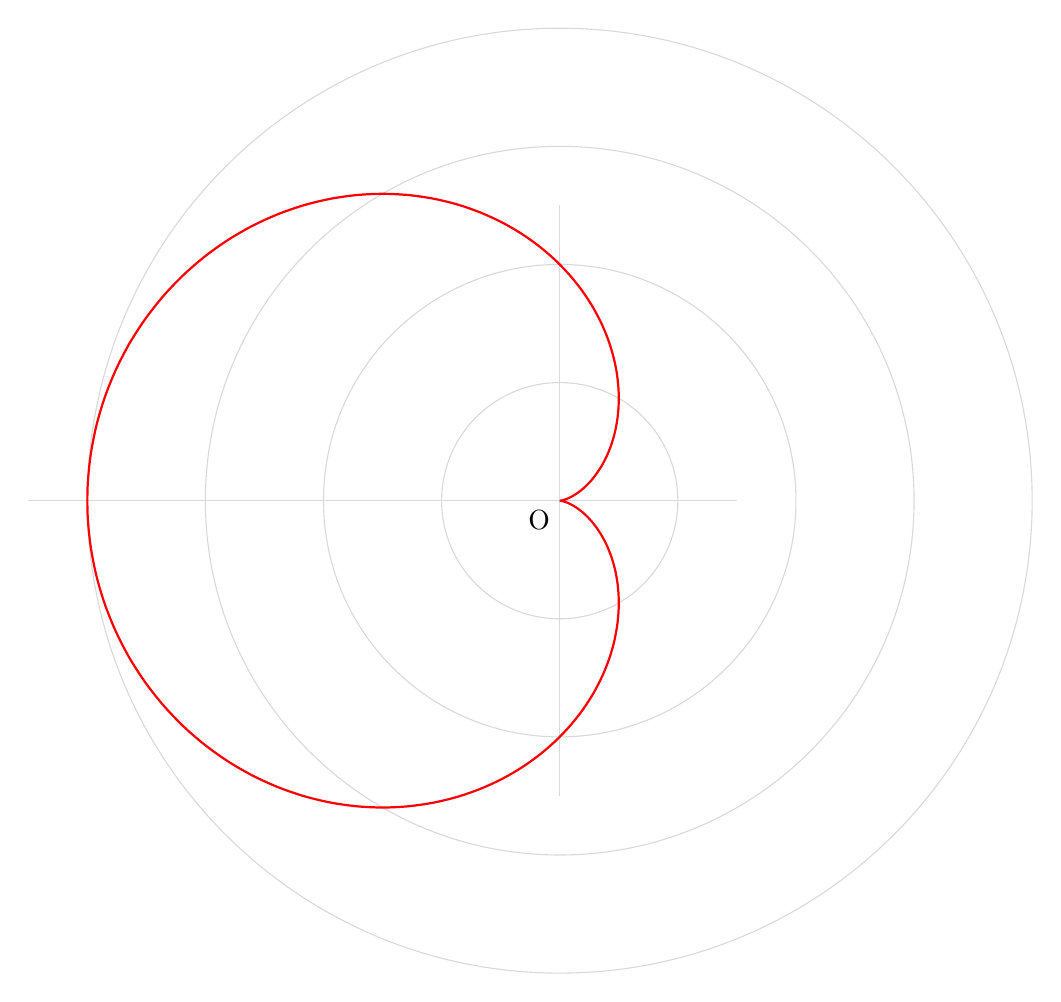
\begin{tikzpicture}[scale=1.5]
    % Draw a simple background grid
    \draw[gray!30, thin] (0,0) circle (1) circle (2) circle (3) circle (4);
    \draw[gray!30, thin] (-4.5,0) -- (1.5,0) (0,-2.5) -- (0,2.5);

    % Plot the cardioid
    % TikZ math engine uses degrees by default
    \draw[thick, red, smooth, samples=100, domain=0:360] 
        plot (\x: {2 - 2*cos(\x)});
        
    % Label the origin
    \node[below left] at (0,0) {O};
\end{tikzpicture}



\begin{question}
In Exercises \ref{polarplotfirst} - \ref{polarplotlast}, plot the graph of the polar equation by hand.  Carefully label your graphs.

\begin{problem} \label{polarplotfirst}
Circle: $r = 6\sin(\theta)$ 
\end{problem}

\begin{problem}
Circle: $r = 2\cos(\theta)$
\end{problem}

\begin{problem}
Rose: $r = 2\sin(2\theta)$ 
\end{problem}

\begin{problem}
Rose: $r = 4\cos(2\theta)$ 
\end{problem}

\begin{problem}
Rose: $r = 5\sin(3\theta)$
\end{problem}

\begin{problem}
Rose: $r = \cos(5\theta)$
\end{problem}

\begin{problem}
Rose: $r = \sin(4\theta)$
\end{problem}

\begin{problem} \label{roseexercise8petal}
Rose: $r = 3\cos(4\theta)$
\end{problem}

\begin{problem}
Cardioid: $r = 3 - 3\cos(\theta)$
\end{problem}

\begin{problem}
Cardioid: $r = 5 + 5\sin(\theta)$
\end{problem}

\begin{problem}
Cardioid: $r = 2 + 2\cos(\theta)$ 
\end{problem}

\begin{problem}
Cardioid: $r = 1 - \sin(\theta)$
\end{problem}

\begin{problem}
Lima\c{c}on: $r = 1 - 2\cos(\theta)$ 
\end{problem}

\begin{problem}
Lima\c{c}on: $r = 1 - 2\sin(\theta)$
\end{problem}

\begin{problem}
Lima\c{c}on: $r = 2\sqrt{3} + 4\cos(\theta)$
\end{problem}

\begin{problem}
Lima\c{c}on: $r = 3-5\cos(\theta)$
\end{problem}

\begin{problem}
Lima\c{c}on: $r = 3-5\sin(\theta)$
\end{problem}

\begin{problem}
Lima\c{c}on: $r = 2 + 7\sin(\theta)$
\end{problem}

\begin{problem}
Lemniscate: $r^{2} = \sin(2\theta)$
\end{problem}

\begin{problem} \label{polarplotlast}
Lemniscate: $r^{2} = 4\cos(2\theta)$ 
\end{problem}

\end{question}

\begin{question}
In Exercises \ref{findpolarintfirst} - \ref{findpolarintlast}, find the exact polar coordinates of the points of intersection of graphs of the polar equations.  Remember to check for intersection at the pole (origin).

\begin{problem} \label{findpolarintfirst}
$r = 3\cos(\theta)$ and $r = 1 + \cos(\theta)$
\end{problem}

\begin{problem}
$r = 1 + \sin(\theta)$ and $r = 1 - \cos(\theta)$
\end{problem}

\begin{problem}
$r = 1-2\sin(\theta)$ and $r=2$
\end{problem}

\begin{problem}
$r = 1 - 2\cos(\theta)$ and $r = 1$
\end{problem}

\begin{problem}
$r = 2\cos(\theta)$ and $r = 2\sqrt{3} \sin(\theta)$
\end{problem}

\begin{problem}
$r = 3\cos(\theta)$ and $r = \sin(\theta)$
\end{problem}

\begin{problem}
$r^2 = 4\cos(2\theta)$ and $r = \sqrt{2}$
\end{problem}

\begin{problem}
$r^{2} = 2\sin(2\theta)$ and $r = 1$
\end{problem}

\begin{problem}
$r = 4\cos(2\theta)$ and $r=2$
\end{problem}

\begin{problem} \label{findpolarintlast}
$r = 2\sin(2\theta)$ and $r = 1$ 
\end{problem} 

\end{question}

\begin{question}
In Exercises \ref{regionsketchfirst} - \ref{regionsketchlast}, sketch the region in the $xy$-plane described by the given set.

\begin{problem}  \label{regionsketchfirst}
$\left\{ (r,\theta) \, | \, 0 \leq r \leq 3, \,0 \leq \theta \leq 2\pi \right\}$
\end{problem}

\begin{problem}
$\left\{ (r,\theta) \, | \, 0 \leq r \leq 4\sin(\theta), \,0 \leq \theta \leq \pi \right\}$
\end{problem}

\begin{problem}
$\left\{ (r,\theta) \, | \, 0 \leq r \leq 3\cos(\theta), \, -\frac{\pi}{2} \leq \theta \leq \frac{\pi}{2} \right\}$
\end{problem}

\begin{problem}
$\left\{ (r,\theta) \, | \, 0 \leq r \leq 2\sin(2\theta), \,0 \leq \theta \leq \frac{\pi}{2} \right\}$
\end{problem}

\begin{problem}
$\left\{ (r,\theta) \, | \, 0 \leq r \leq 4\cos(2\theta), \, -\frac{\pi}{4} \leq \theta \leq \frac{\pi}{4} \right\}$
\end{problem}

\begin{problem}
$\left\{ (r,\theta) \, | \, 1 \leq r \leq 1-2\cos(\theta), \, \frac{\pi}{2} \leq \theta \leq \frac{3\pi}{2} \right\}$
\end{problem}

\begin{problem}
$\left\{ (r,\theta) \, | \, 1 + \cos(\theta) \leq r \leq 3\cos(\theta), \, -\frac{\pi}{3} \leq \theta \leq \frac{\pi}{3} \right\}$
\end{problem}

\begin{problem}
$\left\{ (r,\theta) \, | \, 1 \leq r \leq \sqrt{2\sin(2\theta)}, \, \frac{13\pi}{12} \leq \theta \leq \frac{17\pi}{12} \right\}$
\end{problem}

\begin{problem}
 $\left\{ (r,\theta) \, | \, 0 \leq r \leq 2\sqrt{3} \sin(\theta), \, 0 \leq \theta \leq \frac{\pi}{6} \right\} \cup \left\{ (r,\theta) \, | \, 0 \leq r \leq 2\cos(\theta), \, \frac{\pi}{6}  \leq \theta \leq \frac{\pi}{2} \right\}$
 \end{problem}

\begin{problem} \label{regionsketchlast}
$\left\{ (r,\theta) \, | \, 0 \leq r \leq 2 \sin(2\theta), \, 0 \leq \theta \leq \frac{\pi}{12} \right\} \cup \left\{ (r,\theta) \, | \, 0 \leq r \leq 1, \, \frac{\pi}{12}  \leq \theta \leq \frac{\pi}{4} \right\}$ 
\end{problem}

\end{question}

\begin{question}
In Exercises \ref{setbuildpolarfirst} - \ref{setbuildpolarlast}, use set-builder notation to describe the polar region.  Assume that the region contains its bounding curves.

\begin{problem}\label{setbuildpolarfirst}
The region inside the circle $r = 5$. 
\end{problem}

\begin{problem}
The region inside the circle $r=5$ which lies in Quadrant III.
\end{problem}

\begin{problem}
The region inside the left half of the circle $r = 6\sin(\theta)$.
\end{problem}

\begin{problem}
The region inside the circle $r = 4\cos(\theta)$ which lies in Quadrant IV.
\end{problem}

\begin{problem}
The region inside the top half of the cardioid $r = 3 - 3\cos(\theta)$
\end{problem}

\begin{problem}
The region inside the cardioid $r = 2-2\sin(\theta)$ which lies in Quadrants I and IV.
\end{problem}

\begin{problem}
The inside of the petal of the rose $r = 3\cos(4\theta)$ which lies on the positive $x$-axis
\end{problem}

\begin{problem}
The region inside the circle $r=5$ but outside the circle $r=3$.
\end{problem}

\begin{problem}
The region which lies inside of the circle $r = 3\cos(\theta)$ but outside of the circle $r = \sin(\theta)$
\end{problem}

\begin{problem} \label{setbuildpolarlast}
The region in Quadrant I which lies inside both the circle $r=3$ as well as the rose $r = 6\sin(2\theta)$ 
\end{problem}

\end{question}

\phantomsection
\label{polargraphscalculator}
While the authors truly believe that graphing polar curves by hand is fundamental to your understanding of the polar coordinate system, we would be derelict in our duties if we totally ignored the graphing utility.\footnote{As of this writing, while free online websites and apps like \href{https://www.desmos.com/}{\underline{desmos}} are gaining popularity, the TI-83/84 series calculators are still in wide circulation.} Indeed, there are some important polar curves which are simply too difficult to graph by hand and that makes the calculator an important tool for your further studies in Mathematics, Science and Engineering.  We now give a brief demonstration of how to use the graphing utility to plot polar curves.  The first thing you must do is switch the MODE of your calculator to POL, which stands for ``polar''. 

\begin{center}

\begin{tabular}{ccc}


\includegraphics[width=1.8in]{./PolarGraphsGraphics/Polar01.jpg} &
\hspace{0.05in} 
\includegraphics[width=1.8in]{./PolarGraphsGraphics/Polar02.jpg} & 
\hspace{0.05in} 
\includegraphics[width=1.8in]{./PolarGraphsGraphics/Polar03.jpg} \\

\end{tabular} 

\end{center}

This changes the ``Y='' menu as seen above in the middle.  Let's plot the polar rose given by $r = 3\cos(4\theta)$ from Exercise \ref{roseexercise8petal} above. We type the function into the ``r='' menu as seen above on the right.  We need to set the viewing window so that the curve displays properly, but when we look at the WINDOW menu, we find three extra lines.

\begin{center}

\begin{tabular}{cc}


\includegraphics[width=1.8in]{./PolarGraphsGraphics/Polar04.jpg} &
\hspace{0.75in} 
\includegraphics[width=1.8in]{./PolarGraphsGraphics/Polar05.jpg}\\

\end{tabular} 

\end{center}

In order for the calculator to be able to plot $r = 3\cos(4\theta)$ in the $xy$-plane, we need to tell it not only the dimensions which $x$ and $y$ will assume, but we also what values of $\theta$ to use.  From our previous work, we know that we need $0 \leq \theta \leq 2\pi$, so we enter the data you see above.  (I'll say more about the $\theta$-step in just a moment.)  Hitting GRAPH yields the curve below on the left which doesn't look quite right.  The issue here is that the calculator screen is 96 pixels wide but only 64 pixels tall.  To get a true geometric perspective, we need to hit ZOOM SQUARE (seen below in the middle) to produce a more accurate graph which we present below on the right.  

\begin{center}

\begin{tabular}{ccc}


\includegraphics[width=1.8in]{./PolarGraphsGraphics/Polar06.jpg} &
\hspace{0.05in} 
\includegraphics[width=1.8in]{./PolarGraphsGraphics/Polar07.jpg} & 
\hspace{0.05in} 
\includegraphics[width=1.8in]{./PolarGraphsGraphics/Polar08.jpg} \\

\end{tabular} 

\end{center}

In function mode, the calculator automatically divided the interval [Xmin, Xmax] into 96 equal subintervals.  In polar mode, however, we must specify how to split up the interval [$\theta$min, $\theta$max] using the $\theta$step.  For most graphs, a $\theta$step of 0.1 is fine.  If you make it too small then the calculator takes a long time to graph.  It you make it too big, you get chunky garbage like this.

\begin{center}


\includegraphics[width=1.8in]{./PolarGraphsGraphics/Polar09.jpg} 

\end{center}

You will need to experiment with the settings in order to get a nice graph.  


\begin{question}

Exercises \ref{polarcalcfirst} - \ref{polarcalclast} give you some curves to graph using your calculator.  Note some of them have explicit bounds on $\theta$ and others do not.

\begin{problem} \label{polarcalcfirst}
$r = \theta, \, 0 \leq \theta \leq 12\pi$
\end{problem}

\begin{problem}
$r = \ln(\theta), \, 1 \leq \theta \leq 12\pi$
\end{problem}

\begin{problem}
$r = e^{.1\theta}, \, 0 \leq \theta \leq 12\pi$
\end{problem}

\begin{problem}
$r = \theta^{3} - \theta, \, -1.2 \leq \theta \leq 1.2$
\end{problem}

\begin{problem}
$r = \sin(5\theta) - 3\cos(\theta)$
\end{problem}

\begin{problem}
$r = \sin^{3}\left(\frac{\theta}{2}\right) + \cos^{2}\left(\frac{\theta}{3}\right)$
\end{problem}

\begin{problem}
$r = \arctan(\theta), \, -\pi \leq \theta \leq \pi$ \vphantom{$\frac{1}{1 - \cos(\theta)}$}
\end{problem}

\begin{problem}
$r = \frac{1}{1 - \cos(\theta)}$
\end{problem}

\begin{problem}
$r = \frac{1}{2 - \cos(\theta)}$
\end{problem}

\begin{problem} \label{polarcalclast}
$r = \frac{1}{2 - 3\cos(\theta)}$ 
\end{problem}

\end{question}

\begin{problem}
Use a graphing utility to graph  $r = a - b \sin(\theta)$ for various (positive) values of $a$ and $b$.  Describe the shape of the curve when $a = b$, $a < b$, and when $a > b$.
\end{problem}

 \begin{problem}
 How many petals does the polar rose $r = \sin(2\theta)$ have?  What about $r = \sin(3\theta)$, $r = \sin(4\theta)$ and $r = \sin(5\theta)$?  With the help of your classmates, make a conjecture as to how many petals the polar rose $r = \sin(n\theta)$ has for any natural number $n$.  Replace sine with cosine and repeat the investigation.  How many petals does $r = \cos(n\theta)$ have for each natural number $n$?  
\end{problem}


\begin{question} 
Looking back through the graphs in the section, it's clear that many polar curves enjoy various forms of symmetry.  However, classifying symmetry for polar curves is not as straight-forward as it was for equations back in Section \ref{Relations}.  In Exercises \ref{sympolarfirst} - \ref{sympolarlast}, we have you and your classmates explore some of the more basic forms of symmetry seen in common polar curves.
\phantomsection
\label{polarsymmetry} 


\begin{problem}  \label{sympolarfirst}
Show that if $f$ is even\footnote{Recall that this means $f(-\theta) = f(\theta)$ for $\theta$ in the domain of $f$.} then the graph of $r = f(\theta)$ is symmetric about the $x$-axis.


\begin{enumerate}

\item Show that $f(\theta) = 2 + 4\cos(\theta)$ is even and verify that the graph of  $r = 2+4\cos(\theta)$ is indeed symmetric about the $x$-axis.  (See Example \ref{polargraphex} number \ref{limacon02}.)

\item Show that $f(\theta) = 3\sin\left(\frac{\theta}{2}\right)$ is \textbf{not} even, yet the graph of $r = 3\sin\left(\frac{\theta}{2}\right)$ \textbf{is} symmetric about the $x$-axis.  (See  Example \ref{polargraphintex} number \ref{samepolarcurveex}.) 

\end{enumerate}

\end{problem}

\begin{problem}

Show that if $f$ is odd\footnote{Recall that this means $f(-\theta) = -f(\theta)$ for $\theta$ in the domain of $f$.} then the graph of $r = f(\theta)$ is symmetric about the origin.

\begin{enumerate}

\item  Show that $f(\theta) = 5\sin(2\theta)$ is odd and verify that the graph of $r = 5\sin(2\theta)$ is indeed symmetric about the origin.  (See Example \ref{polargraphex} number \ref{rose}.)

\item  Show that $f(\theta) = 3\cos\left(\frac{\theta}{2}\right)$ is \textbf{not} odd, yet the graph of $r = 3\cos\left(\frac{\theta}{2}\right)$ \textbf{is} symmetric about the origin.  (See  Example \ref{polargraphintex} number \ref{samepolarcurveex}.)

\end{enumerate}

\end{problem}

\begin{problem}
Show that if $ f(\pi-\theta)=f(\theta)$ for all $\theta$ in the domain of $f$ then the graph of $r = f(\theta)$ is symmetric about the $y$-axis. \label{sympolarlast}

\begin{enumerate}

\item  For $f(\theta) = 4-2\sin(\theta)$, show that $f(\pi - \theta) = f(\theta)$ and the graph of $r = 4-2\sin(\theta)$ is symmetric about the $y$-axis, as required.  (See Example \ref{polargraphex} number \ref{limacon01}.)

\item  For $f(\theta) = 5\sin(2\theta)$, show that $f\left(\pi - \frac{\pi}{4} \right) \neq  f\left(  \frac{\pi}{4} \right)$,  yet the graph of $r = 5\sin(2\theta)$ \textbf{is} symmetric about the $y$-axis.  (See  Example \ref{polargraphex} number  \ref{rose}.)

\end{enumerate}

\end{problem}

\end{question}

\begin{question}
In Section \ref{Transformations}, we discussed transformations of graphs.   In Exercise \ref{polargraphtransformations} we have you and your classmates explore transformations of polar graphs. 

\begin{problem} \label{polargraphtransformations}
For Exercises \ref{polargraphexercise1} and \ref{polargraphexercise2} below, let  $f(\theta) = \cos(\theta)$ and $g(\theta) = 2-\sin(\theta)$. 

\begin{enumerate}

\item  \label{polargraphexercise1} Using a graphing utility, compare the graph of $r = f(\theta)$ to each of the graphs of $r = f\left(\theta  + \frac{\pi}{4}\right)$, $r = f\left(\theta  + \frac{3\pi}{4}\right)$, $r = f\left(\theta  - \frac{\pi}{4}\right)$ and $r = f\left(\theta  - \frac{3\pi}{4}\right)$.  Repeat this process for $g(\theta)$.  In general, how do you think the graph of $r = f(\theta + \alpha)$ compares with the graph of $r = f(\theta)$?


\item \label{polargraphexercise2} Using a graphing utility, compare the graph of $r = f(\theta)$ to each of the graphs of $r = 2f\left(\theta\right)$, $r = \frac{1}{2} f\left(\theta\right)$, $r = -f\left(\theta\right)$ and $r = -3 f(\theta)$.  Repeat this process for $g(\theta)$.  In general, how do you think the graph of $r = k \cdot f(\theta)$ compares with the graph of $r = f(\theta)$? 

Follow up question:  does it matter if $k>0$ or $k<0$?

\end{enumerate}

\end{problem}

\end{question}

\begin{problem}
In light of Exercises \ref{sympolarfirst} - \ref{sympolarlast}, how would the graph of $r = f(-\theta)$ compare with the graph of $r = f(\theta)$ for a generic function $f$?  What about the graphs of $r = -f(\theta)$ and $r = f(\theta)$?  What about $r = f(\theta)$ and $r = f(\pi - \theta)$?  Test out your conjectures using a variety of polar functions found in this section with the help of a graphing utility.
\end{problem}

\begin{problem}
With the help of your classmates, research cardioid microphones.
\end{problem}

%\item Back in Section \ref{Relations}, in the paragraph before Exercise \ref{listofcurvesfirst}, we gave you this  \href{http://en.wikipedia.org/wiki/List_of_curves}{\underline{link}} to a fascinating list of curves.  Some of these curves have polar representations which we invite you and your classmates to research.

\end{document}
